\setcounter{chapter}{-1}
\chapter{Introduction}
\label{chap-zero}

% Please add the following required packages to your document preamble:
% \usepackage{booktabs}
% \usepackage{graphicx}
% Please add the following required packages to your document preamble:
% \usepackage{booktabs}
% \usepackage{graphicx}
\begin{table}[]
\caption{\textbf{Key Locations Showing Diverse Phosphorus conditions}}
\label{tab:locations}
\resizebox{\textwidth}{!}{%
\begin{tabular}{@{}lllllllll@{}}
\multicolumn{1}{c}{\textbf{Site}} &
  \multicolumn{1}{c}{\textbf{Relevant Germplasm}} &
  \multicolumn{1}{c}{\textbf{\begin{tabular}[c]{@{}c@{}}Soil\\ pH\end{tabular}}} &
  \multicolumn{3}{c}{\textbf{Soil Phosphorus}} &
  \multicolumn{2}{c}{\textbf{Soil Classification}} &
  \multicolumn{1}{c}{\textbf{Section}} \\ \cmidrule(lr){4-8}
\multicolumn{1}{c}{} &
  \multicolumn{1}{c}{} &
  \multicolumn{1}{c}{} &
  \multicolumn{1}{c}{\textbf{\begin{tabular}[c]{@{}c@{}}ppm\\ (mg/kg)\end{tabular}}} &
  \multicolumn{1}{c}{\textbf{\begin{tabular}[c]{@{}c@{}}Method\\ (notes)\end{tabular}}} &
  \multicolumn{1}{c}{\textbf{Retention}} &
  \multicolumn{1}{c}{\textbf{\begin{tabular}[c]{@{}c@{}}WRB\\ Group\end{tabular}}} &
  \multicolumn{1}{c}{\textbf{\begin{tabular}[c]{@{}c@{}}USDA\\ Order\end{tabular}}} &
  \multicolumn{1}{c}{} \\ \midrule
\begin{tabular}[c]{@{}l@{}}Puerto Vallarta\\ (Bahía de Banderas)\\ Nayarit, México\\ 20°47'2" N 105°14'31" W\end{tabular} &
  \begin{tabular}[c]{@{}l@{}}Grown: \\ PT (MEXI210, AN26)\\ B73\\ PTxB73 RILs\\ AIR (SMS)\end{tabular} &
  7.3 &
  28 &
  Olsen &
  Low &
  Phaeozem &
  Mollisol &
  \begin{tabular}[c]{@{}l@{}}HPC1\\ Kernel Ionomics\end{tabular} \\
 &
   &
   &
   &
   &
   &
   &
   &
   \\
\begin{tabular}[c]{@{}l@{}}Metepec\\ (Toluca)\\ Estado de México, México\\ 19°13'41" N 99°33'1" W\end{tabular} &
  \begin{tabular}[c]{@{}l@{}}Grown:\\ PT (MEXI210, AN26)\\ B73\end{tabular} &
  5.9 &
  91 &
  Bray &
  Low &
  Phaeozem &
  Mollisol &
  HPC1 \\
 &
   &
   &
   &
   &
   &
   &
   &
   \\
\begin{tabular}[c]{@{}l@{}}Ames\\ (Boone)\\ Iowa, USA\\ 42°1'20" N 93°46'36" W\end{tabular} &
  \begin{tabular}[c]{@{}l@{}}Bred: \\ B73\end{tabular} &
  6.2-6.8 &
  13-18 &
  \begin{tabular}[c]{@{}l@{}}Bray\\ (Optimum)\end{tabular} &
  Low &
  Phaeozem &
  Mollisol &
  HPC1 \\
 &
   &
   &
   &
   &
   &
   &
   &
   \\
\begin{tabular}[c]{@{}l@{}}Santa Mónica\\ (Ocuilán)\\ Estado de México, México\\ 18°58'10" N 99°23'57" W\\ 2445 masl\end{tabular} &
  \begin{tabular}[c]{@{}l@{}}Collected:\\ PT (MEXI210, AN26)\end{tabular} &
  6.3 &
  30 &
  Bray &
  Very High &
  Andosol &
  Andisol &
  \begin{tabular}[c]{@{}l@{}}HPC1\\ Kernel ionomics\end{tabular} \\
 &
   &
   &
   &
   &
   &
   &
   &
   \\
\begin{tabular}[c]{@{}l@{}}Rock Springs\\ Pennsylvania, USA\\ 40°42'36" N 77°57'0" W\end{tabular} &
  \begin{tabular}[c]{@{}l@{}}Grown:\\ B73 \\ PTxB73 RILs\\ B73xMICH21 NILs\end{tabular} &
  6.8 &
  \begin{tabular}[c]{@{}l@{}}5 \\ 35\end{tabular} &
  \begin{tabular}[c]{@{}l@{}}Mehlich 3\\ (Low P)\\ (High P)\end{tabular} &
  Low &
  Luvisol &
  Alfisol &
  Inv4m \\
 &
   &
   &
   &
   &
   &
   &
   &
   \\
\begin{tabular}[c]{@{}l@{}}Zacapu\\ Michoacán, México\\ 19°48'0" N 101°47'0" W\\ 2038 masl\end{tabular} &
  \begin{tabular}[c]{@{}l@{}}Collected:\\ MICH21\end{tabular} &
  6.4 &
  54 &
  Bray &
  Very High &
  Andosol &
  Inceptisol &
  Inv4m \\
 &
   &
   &
   &
   &
   &
   &
   &
   \\
\begin{tabular}[c]{@{}l@{}}Santander de Quilichao\\ Cauca, Colombia\\ 3°4'18" N 76°29'54" W\end{tabular} &
  \begin{tabular}[c]{@{}l@{}}Bred:\\ CML530\end{tabular} &
  4.5 &
  5-8 &
  Bray &
  High &
  Acrisol &
  Ultisol &
  Kernel Ionomics \\
 &
   &
   &
   &
   &
   &
   &
   &
   \\
\begin{tabular}[c]{@{}l@{}}Carimagua\\ Meta, Colombia\\ 4°34'25" N 71°20'10" W\end{tabular} &
  \begin{tabular}[c]{@{}l@{}}Grown:\\ CML530\end{tabular} &
  5.2 &
  10 &
  Bray &
  Very high &
  Ferralsol &
  Oxisol &
  Kernel Ionomics \\
 &
   &
   &
   &
   &
   &
   &
   &
   \\
\begin{tabular}[c]{@{}l@{}}Clayton\\ North Carolina, USA\\ 35°40'9" N 78°29'38" W\end{tabular} &
  \begin{tabular}[c]{@{}l@{}}Grown:\\ CML530\\ AIR (TMVB)\end{tabular} &
  6.2 &
  205-622 &
  \begin{tabular}[c]{@{}l@{}}Mehlich 3\\ (Range)\end{tabular} &
  Very high &
  Nitisol &
  Ultisol &
  Kernel Ionomics
\end{tabular}%
}
\end{table}

%% Following sections are examples... not required
%--
\section{Definitions}
\label{sec:def}
%--

Define common terms used throughout the dissertation... 

E.g. African Easterly Waves (AEWs) are waves in the atmosphere over Africa of wavelength ...

%--
\section{Motivations}
\label{sec:mot}
%--

Motivations for studying topic

%--
\section{Background}
\label{sec:back}
%--

Background literature on topic


\begin{figure}[htp]
\centering
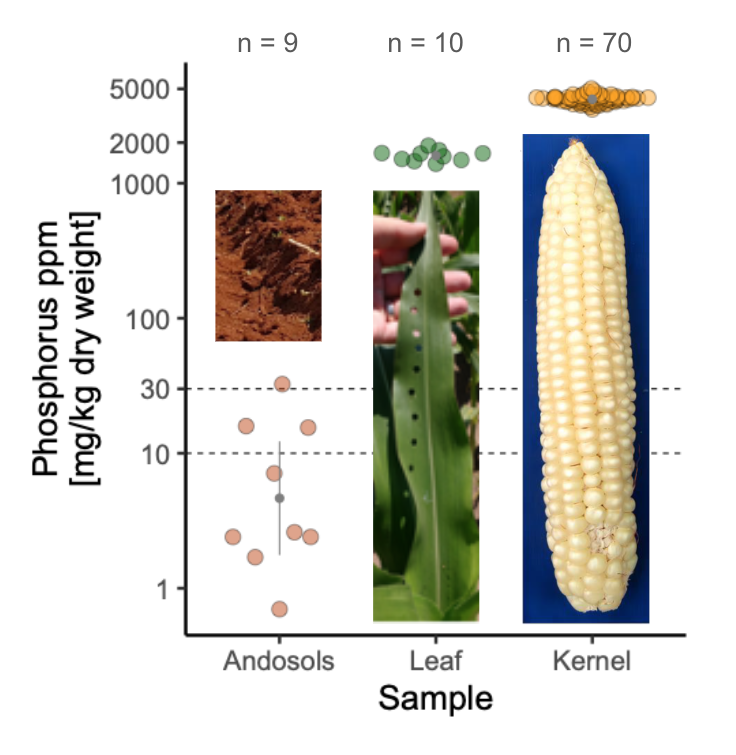
\includegraphics[width=0.5\linewidth]{Chapter-0/figs/P_soil_tissue.png}
\caption[Available phosphorus in soil and total phosphorus in maize tissues]
{\textit{\textbf{Available phosphorus in soil and total phosphorus in maize tissues.}}}
\label{fig::P_soil_tissue}
\end{figure}

%----------
\section{Open Questions and Theories}
\label{sec:que}
%----------

In this section I will present the open questions on the problem I am investigating. 

% \subsection{}
% \label{sec:QTaew-conv}

Background on theories

In summary we will attempt to address the following questions with regard to ...:
\begin{enumerate}
\item Question 1?
\item Question 2?
\item Question 3?
\end{enumerate}
